\documentclass{article}
\usepackage[portuguese]{babel}
\usepackage{graphicx}
\usepackage{listings}
\usepackage[utf8]{inputenc}
\usepackage{listings}
%\graphicspath{ {/home/jessica/Documentos/Engineer/Geocaching-Java} }

\renewcommand{\baselinestretch}{2}
%\author{no realizado por :P}
\title{Geocaching POO}
\date{Junho 2015}


\begin{document}
\maketitle
\begin{center}
Grupo 42 \\
Realizado por: \\
Jéssica Pereira a71164	\\

\includegraphics[height=3\baselineskip,natwidth=369,natheight=430]{jessica0.jpg}\\
Adelino Costa a70563\\
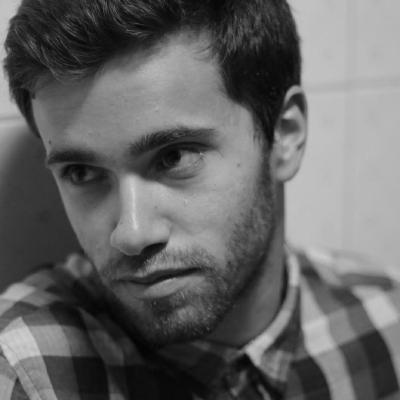
\includegraphics[height=3\baselineskip,natwidth=369,natheight=430]{adelino.jpg}\\
Martinho Aragão a72205 \\

\includegraphics[height=3\baselineskip,natwidth=369,natheight=430]{martinho.jpg}
\end{center}

\pagebreak


\tableofcontents

\pagebreak

\section{Introdução}

\quad
Este trabalho sobre o conceito de Geocaching conhecido nas redes sociais: pretendemos simular
e registar atividades e descobrimentos de caches. Para isso foi necessário modularizar e fazer
as devidas abstrações na preparação para o trabalho, pois quanto mais abstrações forem criadas
mais independentes os módulos serão, podendo depois usar a composição entre estas classes e
fornecendo uma melhor compreensão do código e tratamento da informação.
\par
É necessário o estudo e concepção das classes necessárias, estruturas de dados, métodos
respetivos, variáveis de instância e de classe necessárias, imagina a dependência entre
as classes (composição) e definir uma hierarquia (nomeadamente criando uma super
class para as Caches).
\par Para além de criar classes abstratas, também é necessário guardar todos os dados relativos
às Caches e aos Utilizadores para poder criar métodos eficientes relativos ao tratamento
destes.
\par De entre os requesitos básicos também serão implementados os Eventos, com a simulação
da metereologia e cálculo de distâncias entre caches dados duas coordenadas (coordenadas
iniciais e as coordenadas da cache). Estes dois últimos pontos serão implementados também
em toda a descoberta de Caches/Actividades e não somente no decorrer de Eventos pois serão
úteis nomeadamente para o cálculo de pontuações.
\pagebreak

%Na introdução foram ditos os objetivos. :P

\section{Modularização - Classes criadas}

\quad Decidimos apenas criar 4 tipos de Caches visto a Cache-Evento nao fazer sentido quando temos uma classe que simula eventos, e a Cache Virtual ... 
\par Guardamos todos os users e todas as caches criadas numa base de dados.
\par Para classes que usam estruturas do tipo set criamos vários comparadores úteis para diferentes tipos de ordenação a diferentes classes.
\par Inicialmente tinhamos uma classe chamada 'Server' que acabamos por eliminar pois esta baseia-se na classe GeocachingPOO. A ideia era na classe Server ter acesso a toda a informação, sendo esta apenas acessível aos Admins, mas no próprio GeocachingPOO temos a opção de fazer login como Admin, simplificando e colocando tudo numa classe.
\par Temos hierarquia quanto às caches e quanto aos users.
\par Temos Estatísticas globais, anuais e mensais.
\\
%adicionar imagem do trello final do diagrama
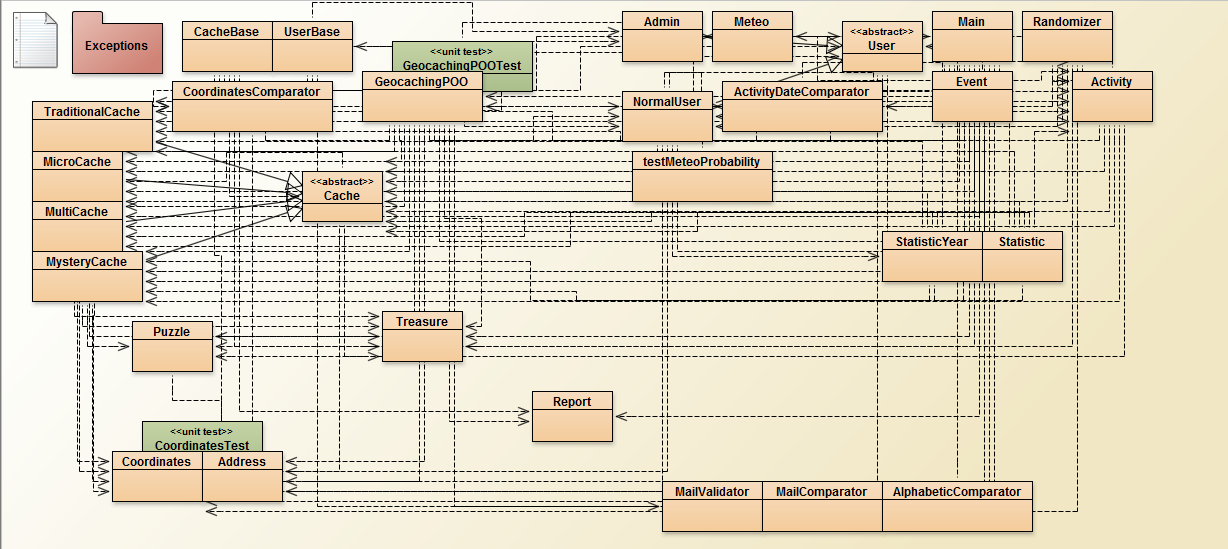
\includegraphics[height=8\baselineskip,natwidth=369,natheight=430]{Diagrama.PNG}

\pagebreak
\section{Bases de dados}

\subsection{CacheBase}
\par Antes de implementarmos a classe \textbf{CacheBase} reflectimos que características únicas teria cada cache para a 
diferenciar de todas as outras.
\par Cada cache tem coordenadas únicas, não sendo possível criar uma cache em coordenadas onde já existe uma cache, 
independentemente do tipo de cache, isto levou-nos a implementar um \textbf{TreeMap} para mapear coordenadas a 
IDs de cache.
\par Para guardar as caches utilizamos um \textbf{ArrayList} visto que sabendo o ID de uma cache é bastante fácil encontrá-lo 
nesta estrutura pois para um dado valor de ID sabemos que a Cache, caso exista, estará no indíce de valor igual a (ID - 1).
\par Portanto a implementação das variáveis de instância de \textbf{CacheBase} é a seguinte:
\begin{lstlisting}[language=Java]
/* ArrayList com as caches */
private ArrayList<Cache> caches;
/* Mapeamento entre e-mails e IDs */
private TreeMap<Coordinates, Double> coords;
\end{lstlisting}

\par Como é necessário um dado Utilizador poder ver as caches que criou utilizamos um \textbf{TreeMap} para mapear 
IDs de Utilizadores a um \textbf{ArrayList} que contém os IDs das caches que o Utilizador criou, caso tenha criado alguma.
\begin{lstlisting}[language=Java]
/* Mapeamento IDs de Utilizadores e IDs de Caches */
private TreeMap<Double, ArrayList<Double>> owners;
\end{lstlisting}

\par Finalmente para implementar o 'report' de Caches criámos outra variável de instância que mapea-se IDs de Caches 
a \textbf{ArrayList} de Reports dessa Cache.
\begin{lstlisting}[language=Java]
/* Mapeamento entre IDs de Caches e Reports dessa cache */
private TreeMap<Double, ArrayList<Report>> reported_caches;
\end{lstlisting}

\newpage
\subsection{UserBase}
\par Para guardar tanto Utilizadores como Administratores primeiros pensamos nas várias maneiras de referenciar um 
Utilizador, assumimos que as maneiras de referenciar um Utilizador seria através do seu ID ou através do seu e-mail.
\par Para os Utilizadores criámos utilizamos um \textbf{TreeMap} que faz o mapeamento de um e-mail para um ID, e 
utilizamos um \textbf{ArrayList} para guardar os Utilizadores pois torna-se bastante rápido encontrar um utilizador dado o
seu ID, visto que para um dado ID o Utilizador, caso exista, estará no indice de valor igual a (ID - 1) no \textbf{ArrayList}.
\par Ficaram então definidas desta forma as variáveis de instância de \textbf{UserBase}:
\begin{lstlisting}[language=Java]
/* ArrayList com os utilizadores */
private ArrayList<NormalUser> users;
/* Mapeamento entre e-mails e IDs */
private TreeMap<String, Double> userMails;
\end{lstlisting}

\par Para guardar as várias instâncias de \textbf{Admin} utilizamos o mesmo método que no caso das instâncias de
\textbf{NormalUser}. Segue-se a definição das variáveis de instância:
\begin{lstlisting}[language=Java]
/* ArrayList com os administradores */
private ArrayList<Admin> admins;
/* Mapeamento entre e-mails e IDs */
private TreeMap<String, Double> adminMails;
\end{lstlisting}













\pagebreak

TODO
\section{ Caches }
Como criamos uma Cache?
Como tratamos da Invalidação de uma Cache?
Como permitirmos ao user para reportar uma cache e quando é que ela é efetivamente reportada? pelo admin... 

Mencionar que Cache é superclasse e os tipos de cache são sub-classes Estrutura de cada uma;

Ao fazer report de uma cache o admin tem acesso a essas caches e pode remover essa cache aceitando o report ou eliminar esse report. Se o utilizador remover a cache (invalidando-a) depois de ter feito report a essa cache, quando voltamos para o contexto do admin, essa cache já nao existe nos reports porque foi eliminada.

\subsection{ Cache Tradicional}
\subsection{ Micro Cache }
\subsection{ Multi Cache}
\subsection{ Cache Mistério }



\pagebreak
\section{Register e Login}
TODO
Falar no user e o que ele pode fazer : atividades, registos de estatisticas, amigos...
registo dos seus amigos falar onde diz TODO AMIGOS

Ao iniciar o programa, o user efetua o seu registo com e-mail, pass, nome, morada etc... Quando faz login é-lhe apresentado a sua pontuação a 0 ao lado do seu nome, e um menu inicial.
Neste menu, o user pode ver as caches que estão a uma dada distância da sua localização (fornecendo coordenadas ao programa/ aplicação), identificadas pelo seu id. Pode criar caches dos 4 tipos existentes, adicionar uma atividade, fazer pedidos de amizade, entre outros requisitos básicos explicitos no enunciado.

Este login usa uma encriptação da pass tornando a informação do user segura e tornando este programa mais realísta.








\pagebreak
\section{Atividades e Estatísticas}

\subsection{Atividades}
\quad Quando o user encontra uma cache, regista uma nova Atividade que é automaticamente adicionada às Estatísticas.
\par Esta atividade têm como informações a data em que foi adicinada, a Cache que foi encontrada, os kilometros que foram percorridos para encontrar esta Cache, a pontuação ganha pelo feito e a Meteorologia desse dia.
\par O utilizador apenas tem de fornecer os dados quanto à Cache que encontrou e em que dia foi. O resto é tratado pelo programa, havendo simulações e cálculos.

\subsubsection{Kilómetros}
\quad  Quando adiciona a primeira atividade, são criadas as coordenadas iniciais do local onde o User iniciou a procura, geradas aleatóriamente fazendo cópia das coordenadas da Cache e um incremento da latitude e longitude de valores entre 0,001 e 0,4 por exemplo. No momento em que, ao adicionar esta primeira atividade, o programa calcula as distâncias entre estas coordenadas geradas aleatóriamente com base neste range, e as coordenadas da Cache, os kilometros calculados dão entre valores de 0,1km até 40 kms, em média.
Este incremento de latitude e longitude são métodos que usam o Math.Random, presentes na classe "Coordinates".
\par Caso já exista uma atividade anterior a esta que está prestes a ser adicionada, a distância calculada será entre as coordenadas desta cache e as coordenadas da cache da ultima atividade, tornando isto o mais realista possivel. A última atividade é a última posição conhecida do utilizador.
\\


\subsubsection{Meteorologia}
\quad  Na classe Meteo são geradas as meteorologias de uma forma aleatória também. Existem dois campos que dizem respeito à Temperatura e ao Estado de Tempo. 
\par int Low = -10;
\par int High = 40;
\par São definidos os valores mínimos e máximos para a Temperatura. Para a Weather existem 7 tipos possíveis que são os seguintes:
\par Rainy 0
\par Stormy 1
\par Sunny 2
\par Cloudy 3
\par Windy 4
\par Foggy 5
\par Hail 6
\par A cada estado de tempo está associado um número que vai ser gerado aleatóriamente com o Math.Random entre os valores de inteiros de 0 até 7 (exclusive).
\\

\par Tudo isto é muito importante para as Estatísticas pois são calculados os pontos em cada Atividade, conforme o estado de tempo, os kilometros percorridos e o tipo de cache encontrada. 
\par Para cada atividade existe um limite de pontos que decidimos atribuir: 100 pontos. Assim se quisermos diminuir ou aumentar este limite é só tratar da escala deste limite que será mais fácil. (Por exemplo, para cada atividade apenas querer 10 pontos, ou querer 1000, etc. ...).
\par Este limite de pontos total rege-se também por um limite às 3 atribuiçoes de pontos que criamos,  kilometros, meteorologia e cache, que são apresentados de seguida:
\begin{lstlisting}
private static int limit_points = 100;
private static int limit_points_cache = 50;
private static int limit_points_kms = 30;
private static int limit_points_meteo = 20;
\end{lstlisting}

\par * Decidimos atribuir mais pontos ao fator do tipo da cache. Se for uma Micro Cache atribuimos o mínimo de pontos (10) mas se for uma Mystery Cache o user consegue obter os 50 pontos máximos, dependendo também da dificuldade do Puzzle que foi atribuida. Como a estrela de dificuldade vai de 1 a 10, decidimos atribuir dificuldade * 5 pontos pela Mystery Cache.
\par Da mesma forma, tomamos decisões para o cálculo de pontos da Meteorologia e dos kilometros. Se percorrer mais kilómetros, ganha mais pontos e se o tempo estiver mau (Stormy, Hail ...) atribuimos o máximo de pontos para a Weather que são 10 pontos. Não esquecer que também temos a Temperatura, e para o caso de temperaturas extremas (muito baixas e muito altas) atribuimos também pontuações máximas. Depois, para cada situação à uma atribuição mediana conforme a meteorologia e temperatura.

TODO CODIGO A SER FEITO
\par O user tem possibilidade de visualizar as 10 últimas Atividades tanto dele como dos amigos, e de, se assim o quiser, as remover. Quando remove uma atividade, todas as informações e pontos adquiridos por esta são automaticamente retirados das estatisticas.


\subsection{Estatísticas}
\quad Quando às Estatísticas temos duas classes: StatisticYear e Statistic.
A razão pela qual temos duas classes é porque decidimos guardar também as Estatísticas Globais do user, ou seja, as estatísticas de todos os anos. Para melhor entender o funcionamento e a estrutura destas classes, começaremos por explicar a Statistic.

\par Na Statistic temos as estatísticas de um dado ano. A estrutura é a seguinte:
\begin{lstlisting} 
ArrayList < TreeSet<Activity>>. 
\end{lstlisting}

Tentamos criar um array para ter em cada indice o mês ligado ao conjunto de atividades desse mês mas é impossivel criar array com valores que não sejam primitivos, logo tivemos de mudar a estrutura para um ArrayList. Este ArrayList terá como indices o mês da estatistica. O seu conteúdo será o conjunto de Atividades realizadas nesse mês. Para adicionar uma atividade garantimos que não é possivel adicionar uma atividade se o ano não for o mesmo. Por isso é importante buscar o ano desta estatística, fazer set do ano desta estatística... O ano assumido como default é o current year que é 2015. Também são disponibilizadas funções como o de contar quantos tipos de cache num dado mês existem, e devolver num array, soma de pontos, de kms totais, numero de todas as caches encontradas, tanto para este ano como para um dado mês. Estas função são usadas como auxiliares na classe StatisticYear, e o porquê será entendido em seguida, quando for explicada a estrutuda da mesma.
\par StatisticYear é basicamente uma estrutura que mapeia um dado ano para uma Statistic. É esta a estrutura usada no programa pois facilmente se adiciona uma atividade nesta estrutuda, tendo o ano em que queremos inserir na data da atividade e usando os métodos existentes no Statistic como auxiliares. Todo o resto sobre o numero total de pontos, kilometros percorridos, numero de caches, etc... também são fornecidos por métodos de assinaturas iguais (tirando partido do Overloading), tanto para um dado ano como para todos os anos (global).


\par Permitimos ao user ver as suas estatiticas globais, anuais (de um dado ano) e mensais. Para as estatisticas mensais assumimos que ele quer ver um dado mês do current year (2015). Mas tal pode ser alterado facilmente, pedindo apenas mais uma informação extra ao user (que ano quer) antes de mostrar informações destas estatísticas.

\par Existe ainda uma opção para ver um gráfico de quantas caches dos tipos existentes o usuário encontrou, num dado mês.




\pagebreak
TODO AMIGOS
\section{Amigos}
Pedidos de amizade, ver atividades dele, etc ....




\pagebreak
\section{Eventos}
TODO










\pagebreak
\section{Programa Principal e Main}
\quad Na classe \textbf{GeocachingPOO} estão as chamadas de todos os métodos existentes em todas as classes que 
permitem uma interação a nível de Objetos.

\par No Main estão todos os Menus e toda a interação I/O entre o utilizador e o nosso programa. sCom isto permitimos que o nosso programa possa ser implementado com outras Interfaces Gráficas, nomeadamente para a 
web, etc. ...




\pagebreak
\section{Salvaguarda do Estado e Load do último Estado}
TODO explain how this works




\pagebreak
\section{Tratamento de Excepções}
\quad Decidimos colocar todas as excepções num package chamado Exceptions para uma melhor visualização das classes e 
clareza no diagrama. Para todas as classes que implementam Excepções é feito import deste Package. Apenas a função 
\em main faz o tratamento de Excepções.
\pagebreak
\section{Conclusão}




\end{document}